%%%%%%%%%%%%%%%%%%%%%%%%%%%%%%%%%%%%%%%%%
% This template originates from:
% http://www.LaTeXTemplates.com
%%%%%%%%%%%%%%%%%%%%%%%%%%%%%%%%%%%%%%%%%

%----------------------------------------------------------------------------------------
%	PACKAGES AND OTHER DOCUMENT CONFIGURATIONS
%----------------------------------------------------------------------------------------

\documentclass[11pt]{scrartcl} % Font size

%%%%%%%%%%%%%%%%%%%%%%%%%%%%%%%%%%%%%%%%%
% This template originates from:
% http://www.LaTeXTemplates.com
%%%%%%%%%%%%%%%%%%%%%%%%%%%%%%%%%%%%%%%%%

%----------------------------------------------------------------------------------------
%	PACKAGES AND OTHER DOCUMENT CONFIGURATIONS
%----------------------------------------------------------------------------------------
\usepackage{xcolor}
\usepackage{amsmath, amsfonts, amsthm} % Math packages
\usepackage{minted}
\usepackage{listings} % Code listings, with syntax highlighting
% Umbenennung von Listing auf Auflistung
\renewcommand\listoflistingscaption{Auflistungen}
\usepackage{caption}
\DeclareCaptionLabelFormat{Auflistung}{#1 #2}
\captionsetup[listing]{labelformat=Auflistung, name=Auflistung}


\usepackage{pdflscape}
\usepackage{float} % Enables [H] positioning option for figures

\usepackage[ngerman]{babel} % English language hyphenation
\usepackage{tabularx}
\usepackage{graphicx} % Required for inserting images
\usepackage{hyperref} % for hyperlinks
\providecommand*{\listingautorefname}{Auflistung}
\graphicspath{{Figures/}{./}} % Specifies where to look for included images (trailing slash required)

\usepackage{booktabs} % Required for better horizontal rules in tables

\numberwithin{equation}{section} % Number equations within sections (i.e. 1.1, 1.2, 2.1, 2.2 instead of 1, 2, 3, 4)
\numberwithin{figure}{section} % Number figures within sections (i.e. 1.1, 1.2, 2.1, 2.2 instead of 1, 2, 3, 4)
\numberwithin{table}{section} % Number tables within sections (i.e. 1.1, 1.2, 2.1, 2.2 instead of 1, 2, 3, 4)
\numberwithin{listing}{section} % Number tables within sections (i.e. 1.1, 1.2, 2.1, 2.2 instead of 1, 2, 3, 4)

\setlength\parindent{0pt} % Removes all indentation from paragraphs

\usepackage{enumitem} % Required for list customisation
\setlist{noitemsep} % No spacing between list items

\usepackage{color}

\definecolor{pblue}{rgb}{0.13,0.13,1}
\definecolor{pgreen}{rgb}{0.0,0.5,0}
\definecolor{pred}{rgb}{0.9,0,0}
\definecolor{pgrey}{rgb}{0.46,0.45,48}

%----------------------------------------------------------------------------------------
%	DOCUMENT MARGINS
%----------------------------------------------------------------------------------------

\usepackage{geometry} % Required for adjusting page dimensions and margins

\geometry{
	paper=a4paper, % Paper size, change to letterpaper for US letter size
	top=2.5cm, % Top margin
	bottom=3cm, % Bottom margin
	left=3cm, % Left margin
	right=3cm, % Right margin
	headheight=0.75cm, % Header height
	footskip=1.5cm, % Space from the bottom margin to the baseline of the footer
	headsep=0.75cm, % Space from the top margin to the baseline of the header
	%showframe, % Uncomment to show how the type block is set on the page
}

%----------------------------------------------------------------------------------------
%	FONTS
%----------------------------------------------------------------------------------------

\usepackage[utf8]{inputenc} % Required for inputting international characters
\usepackage[T1]{fontenc} % Use 8-bit encoding

\usepackage{fourier} % Use the Adobe Utopia font for the document

%----------------------------------------------------------------------------------------
%	SECTION TITLES
%----------------------------------------------------------------------------------------

\usepackage{sectsty} % Allows customising section commands

\sectionfont{\vspace{6pt}\normalfont\scshape} % \section{} styling
\subsectionfont{\normalfont\bfseries} % \subsection{} styling
\subsubsectionfont{\normalfont\itshape} % \subsubsection{} styling
\paragraphfont{\normalfont\scshape} % \paragraph{} styling

\usepackage[titles]{tocloft} %customizable table of content

%----------------------------------------------------------------------------------------
%	Hyper Links Setup - Definition of the different links styles
%----------------------------------------------------------------------------------------
\hypersetup{
    colorlinks=true,
    linkcolor=black,
    filecolor=magenta,      
    urlcolor=cyan,
    citecolor=blue,
}

%----------------------------------------------------------------------------------------
%	HEADERS AND FOOTERS
%----------------------------------------------------------------------------------------
\usepackage{fancyhdr}% Required for customising headers and footers
\usepackage[lastpage, user]{zref}
\fancyhf{}
\lhead{HSLU Datenbanksysteme} % Left header
\rhead{Team 4} % right header
%\lfoot{\today} % left footer %% Comment Oli: M.M nach nicht relevant auf jeder Seite
%\rfoot{\thepage/\zpageref{LastPage}} % right footer
\renewcommand{\headrulewidth}{0.5pt}
\renewcommand{\footrulewidth}{0.5pt}
%\usepackage{scrlayer-scrpage} % Required for customising headers and footers

%\ohead*{} % Right header
%\ihead*{} % Left header
%\chead*{} % Centre header

%\ofoot*{} % Right footer
%\ifoot*{} % Left footer
%\cfoot*{\pagemark} % Centre footer

%----------------------------------------------------------------------------------------
%	JAVA CODE STYLE
%----------------------------------------------------------------------------------------

\lstdefinestyle{javaCodeStyle}{
	language=Java, % Use Java functions/syntax highlighting
	frame=single, % Frame around the code listing
	showspaces=false,
	showtabs=false,
	breakatwhitespace=true,
	breaklines=true,
	postbreak=\mbox{\textcolor{red}{$\hookrightarrow$}\space},
	commentstyle=\color{pgreen},
	keywordstyle=\color{pblue},
	stringstyle=\color{pred},	
	basicstyle=\scriptsize,
	showstringspaces=false, % Don't put marks in string spaces
	numbers=left, % Line numbers on left
	numberstyle=\tiny, % Line numbers styling
}

\lstset{style=javaCodeStyle}


\usepackage{minted}
%----------------------------------------------------------------------------------------
%	New Commands
%----------------------------------------------------------------------------------------
%Define texttt with hyphenation enabled
\DeclareTextFontCommand{\mytexttt}{\ttfamily\hyphenchar\font=45\relax}

%For code in text
\newcommand{\code}[1]{\mytexttt{#1}}

%Prevent dots in TOC
\renewcommand{\cftdot}{}

%SubItem for Itemize
\newcommand{\subItem}[1]{
    {\setlength\itemindent{15pt} \item[-] #1}
}


\usepackage[style=numeric,sorting=none]{biblatex}
\usepackage{csquotes}

\usepackage{tcolorbox}
 % Include the file specifying the document structure and custom commands


%----------------------------------------------------------------------------------------
%	TITLE SECTION
%----------------------------------------------------------------------------------------
\title{	
	\begin{figure}[h]
		\begin{flushright}
			
\includegraphics[width=0.2\textwidth]{bilder/hsluLogo.eps}			
		\end{flushright}
	\end{figure}
	\vspace{40pt} % Whitespace
	\normalfont\normalsize
	\textsc{Hochschule Luzern - Informatik}
	\vspace{25pt} % Whitespace
	\rule{\linewidth}{0.5pt}\\ % Thin top horizontal rule
	{\huge Software Testing (SWT)}\\ % The assignment title
	\vspace{10pt} % Whitespace	
	{\large Zusammenfassung von Oliver Amstutz, \today }
	\vspace{12pt} % Whitespace
	\rule{\linewidth}{0.5pt}\\ % Thin top horizontal rule
	\vspace{12pt} % Whitespace
}

\addbibresource{bibtex/refs.bib}

%für pagebreak in Anhang
\newenvironment{longlisting}{\captionsetup{type=listing}}{}

\begin{document}

\pagenumbering{roman}
\rfoot{\thepage} % right footer

%To remove dots in Auflistungen
\makeatletter
\renewcommand\@dotsep{10000}
\makeatother

\maketitle % Print the title
\pagestyle{fancy}
\thispagestyle{empty}
\newpage
\setcounter{page}{1}


\newpage
\tableofcontents
%\newpage
%\listoffigures
%\listoftables
% \renewcommand{\cftdotsep}{\cftnodots}
%\listoflistings

\newpage
\rfoot{\thepage/\zpageref{LastPage}} % right footer
\pagenumbering{arabic}
\section{SW01}

\subsection{Getestet wird immer}
\label{subsec: Getestet wird immer}
Getestet wird immer, es bleibt nur offen:
\begin{itemize}
    \item Wann wird getestet?
    \item Wer testet?
    \item Wo werden die Test Resultate veröffentlicht?
\end{itemize}
Es lohnt sich das Testen vor der Entwicklung einzuplanen (Kosten, Zeitpunkt, Image Schaden).
Beispiele sind:
\begin{itemize}
    \item Unzureichender Last-Test für Ski-Gebiete Online Buchung
    \item Sirenentest musste wegen Systemfehler wiederholt werden 
    \item Oberflächenbehandlungsmaschine welche bereits mit ungenügenden Test geplant wurde (Funktion Düsen nicht interdisziplinär getestet, Positionsensor nicht auf voller Leistung getestet wegen Lärm)
\end{itemize}

\subsection{Die 10er Regel}

Die Abbildung \ref{fig:10er Regel} besagt, dass je weiter ein Fehler sich unentdeckt in die späteren Phasen des Werdeganges eines Produktes oder Prozesses bewegt, umso höher werden die Kosten zur Behebung dieses Fehlers~\cite{sixsigmablackbelt.de}.

\begin{figure}[H]
	\centering
	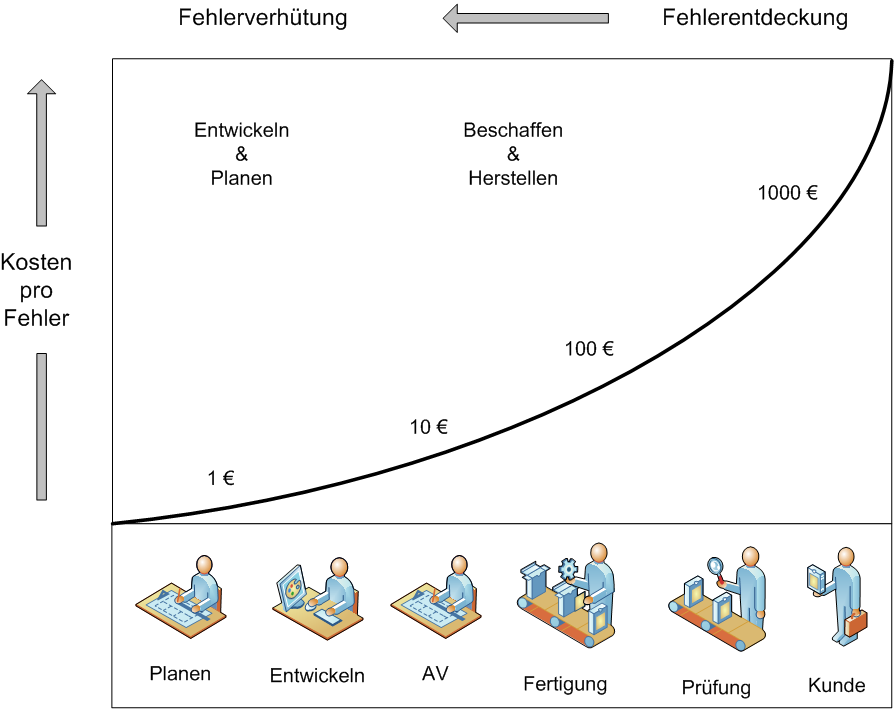
\includegraphics[width=1.0\columnwidth]{01/bilder/Fehlerkosten-10-er-Regel.png}
	\caption{Fehler-kosten der 10er Regel (rule of ten).}
	\label{fig:10er Regel}
\end{figure}

Beispiele:
\begin{itemize}
    \item Beispiele aus Unterkapitel \ref{subsec: Getestet wird immer}
    \item Heroes of Newearth Game-Entwicklung: nicht-Initialisierung einer Variable hat im 64Bit System zum Fehler geführt, welches erst beim Release durch die User bemerkt wurde. Rollback war notwendig.
\end{itemize}

Je früher ein Fehler erkannt wird, desto billiger ist die Behebung!

\subsection{Testen bringt Nutzen}
Mehr Qualität:
\begin{itemize}
    \item wird messbar und quantifizierbar und dadurch sichtbar und verkaufbar
    \item was messbar ist, wird steuerbar
    \item kann somit gezielt gesteigert werden
\end{itemize}

Mehr Wirtschaftlichkeit:
\begin{itemize}
    \item Frühes Erkennen von Fehler ist billiger
    \item After Sales Support wird weniger (Einsparen von Kosten)
    \item Testen dokumentiert Wissen und schützt so Investitionen
    \item Ressourcen werden sinnvoll eingesetzt
\end{itemize}

Risikomanagement:
\begin{itemize}
    \item Risiken werden frühzeitig identifiziert
    \item Risiken werden aktiv gemanagt
    \item Das Eintreffen der Risiken kann vermieden werden
    \item Es wird dort getestet, wo es sinnvoll ist (in der Regel wird das getestet was man: kennt, schon immer getestet hat, gut bekannt ist)
\end{itemize}

Besserer Wettbewerbsvorteil:
\begin{itemize}
    \item keine negativ Presse
    \item hohe Reputation dank Zuverlässigkeit
    \item Erweiterbarkeit und Wartbarkeit ergeben Nachhaltigkeit
    \item swissness, Qualitätsbewusstsein
\end{itemize}


\subsection{Testqualität vs. Produktqualität}
Abbildung \ref{fig: Testqualität vs. Produktqualität} zeigt auf der X-Achse die Testqualität und auf der Y-Achse die Produktqualität~\cite{theNoserWayOfTesting}.

\begin{figure}[H]
	\centering
	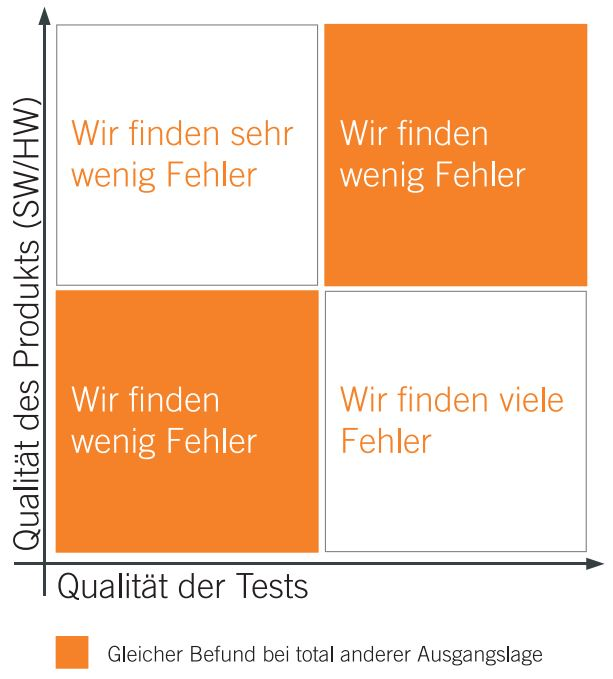
\includegraphics[width=0.6\columnwidth]{01/bilder/Testqualität vs Produktqualität.JPG}
	\caption{Testqualität gegenüber Produktqualität.}
	\label{fig: Testqualität vs. Produktqualität}
\end{figure}

Aus der Abbildung lassen sich folgende Rückschlüsse ziehen:
\begin{itemize}
    \item Testqualität ist entscheidend, nur "halbes Testing" bringt nichts!
    \item Der Grund fürs Testen ist es herauszufinden ob man eine gute oder schlechte Produktqualität hat.
    \item Ist die Testqualität schlecht, können keine Rückschlüsse auf die Produktqualität gewonnen werden -> Provokativ: Warum testet man dann überhaupt?
    \item Man findet sehr wenig Fehler -> gute Entwickler, schlechte Tester
    \item Man findet sehr viele Fehler -> schlechte Entwickler, gute Tester
    \item Aufpassen da man den gleichen Befund haben kann bei total unterschiedlicher Ausgangslage!
    \item Je besser das Testen, desto schlechter erscheint die Produktqualität
    \item Als Konsequenz kann man also sagen - nur die besten testen!
\end{itemize}

Das Bewerten der Fehlerzahl kann über das Messen der gefundenen Fehler im Verlaufe des Projektes bewertet werden. Abbildung \ref{fig: Fehlerkumulation über die Zeit} zeigt das Aufkumulieren der Fehler über die Zeit. Die X-Achse ist die Zeit, die Y-Achse sind alle gefundenen Fehler.

\begin{figure}[H]
	\centering
	\includegraphics[width=0.4\columnwidth]{01/bilder/Fehlerkumulation über die Zeit.JPG}
	\caption{Fehlerkumulation eines SW-Produktes über die Zeit.}
	\label{fig: Fehlerkumulation über die Zeit}
\end{figure}

Wenn der Gradient der gefundenen Fehler (rote Linien) flacher wird, ist dies ein Zeichen dafür, das mit den angewandten Methoden keine weiteren Fehler gefunden werden können. Das kann auch so interpretiert werden, das in Abbildung \ref{fig: Testqualität vs. Produktqualität} man die Qualität des Produktes gesteigert hat. Das sich die Qualität der Tests verschlechter über Zeit wird nicht angenommen.
Weitere Info's zu diesem Thema in Kapitel \textcolor{red}{Noch zu definieren - später!}.

\subsection{Anforderungen der Stakeholder}
Stellen Sie sich ein Glas / Ball vor. Ich kann ein Glas/Ball nicht testen ohne die Anforderungen der Stakeholder zu kennen. Dies beinhaltet:
\begin{itemize}
    \item Anwendungszweck
    \item Umgebung
    \item Bedürfnisse
    \item Kontext
\end{itemize}

Ein Softwaretest prüft und bewertet Software auf Erfüllung der für ihren Einsatz definierten Anforderungen und misst ihre Qualität. Fürs Testen braucht's Erwartungen, Anforderungen und Akzeptanzkriterien!

\textcolor{red}{Noch am passenden Ort einfüllen:}
Code qualität bei der Entwicklung bereits prüfen mit:
\begin{itemize}
    \item 4 Augen Prinzip
    \item Codereview
    \item Pair-Programming
\end{itemize}

Die erste Teststufe liegt bereits beim Software Entwickler!

%\section{Datenmanagement}
In diesem Kapitel wird der Use-Case vorgestellt. Anschliessend wird die für die  Abwicklung des Use-Case benötigte Datenarchitektur beschrieben. Die ausgewählte Datenbank Technologie, sowie die Projektarchitektur sind in den letzten zwei Unterkapiteln ersichtlich.


\subsection{Use-Case}
\label{subsec: use case}

Das Projektteam hat sich dazu entschieden, Daten von Filmen zu analysieren, um den folgenden Use-Case zu bearbeiten:
\\
Ein Investor möchte einen neuen Blockbuster im Genre der Action-Filme in die Kinos bringen. Das Zielpublikum sind alle Personen, die zwischen 18 und 30 Jahre alt sind. Ziel des Investors ist ein möglichst erfolgreicher Film in einer bestimmten Kultur\footnote{Beispielsweise Hollywood hat als Produktionsland (zukünftig als Land abgekürzt) die USA, Bollywood hat Indien.}. Um dies zu erreichen, ist er auf der Suche nach dem perfekten Filmteam. Dieses Team soll sich aus folgenden Rollen zusammensetzen:
\begin{itemize}
	\item ein Produzent
	\item ein Drehbuchautor
	\item ein Regisseur
	\item drei Schauspieler
	\item drei Schauspielerinnen
\end{itemize}

Daraus ergibt sich folgende Entscheidungsfrage:\\
\begin{tcolorbox}
    Welches Filmteam soll angeheuert werden, um den grösstmöglichen Erfolg beim genannten Zielpublikum zu erreichen?
\end{tcolorbox}

Für die Beantwortung der Use-Case Entscheidungsfrage muss die Komplexität der Realität reduziert werden. Dies wird über Annahmen und Vereinfachungen erreicht. Beispielsweise werden die jeweiligen Filmrollen isoliert betrachtet. Für ein objektives Bewerten der erbrachten Leistung einer Person müssen Bewertungskriterien eingeführt werden. Mit einem oder wenigen Performance Parametern können schliesslich die einzelnen Personen in ihren Rollen miteinander verglichen und bewertet werden.


\subsection{Datenarchitektur}
Eine geeignete Datenstruktur ist notwendig für das erfolgreiche Auswerten des Use-Cases. \autoref{fig:Datenarchitekur} zeigt die notwendige Datenstruktur mit den entsprechenden Attributen. 

\begin{figure}[H]
	\centering
	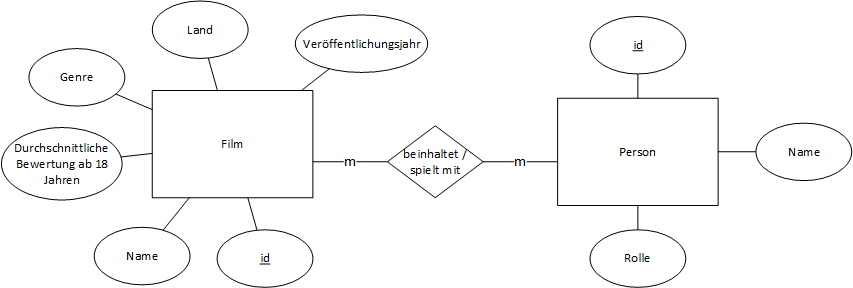
\includegraphics[width=1.0\columnwidth]{2_Datenmanagement/Bilder/Datenarchitektur.png}
	\caption{Datenarchitektur des Use-Cases.}
	\label{fig:Datenarchitekur}
\end{figure}

\subsection{Datenbanktechnologie}

Für diese Anwendung wird eine \textit{MySQL} Datenbanktechnologie verwendet. Folgende Argumente sprechen für die Wahl von \textit{MySQL}:
\begin{itemize}
	\item Weit verbreitete Technologie~\cite{db-engines.com} mit umfangreicher Community.
	\item Das Volumen der Datenbasis ist in der Megabyte-Grössenordnung. Dementsprechend eignet sich ein bewährtes relationales Datenbanksystem.
	\item Das Arbeiten mit Metadaten in Tabellen bietet sich für die Datenbasis an. Die Vorteile von No-SQL Datenbanksystemen sind beim gegebenen Datensatz unbedeutend.
\end{itemize}

\subsection{Projektarchitektur}
Um die nachfolgenden Beschreibungen sowie Erläuterungen besser zu verstehen, wird in diesem Unterkapitel die gesamte Architektur des Projekts dargestellt. Die \autoref{fig:Projektarchitektur} zeigt diese Architektur unterteilt in mehreren Schichten. Die eigentlichen Datenbank-Operationen finden auf der Daten-Schicht statt. Die Aufbereitung der Abfragen wird in der Schicht der Business-Logik durchgeführt. Schliesslich werden in der Präsentations-Schicht die Resultate als auch die Abfragemöglichkeiten über einen Webserver auf einer Webseite dargestellt.

\begin{figure}[H]
	\centering
	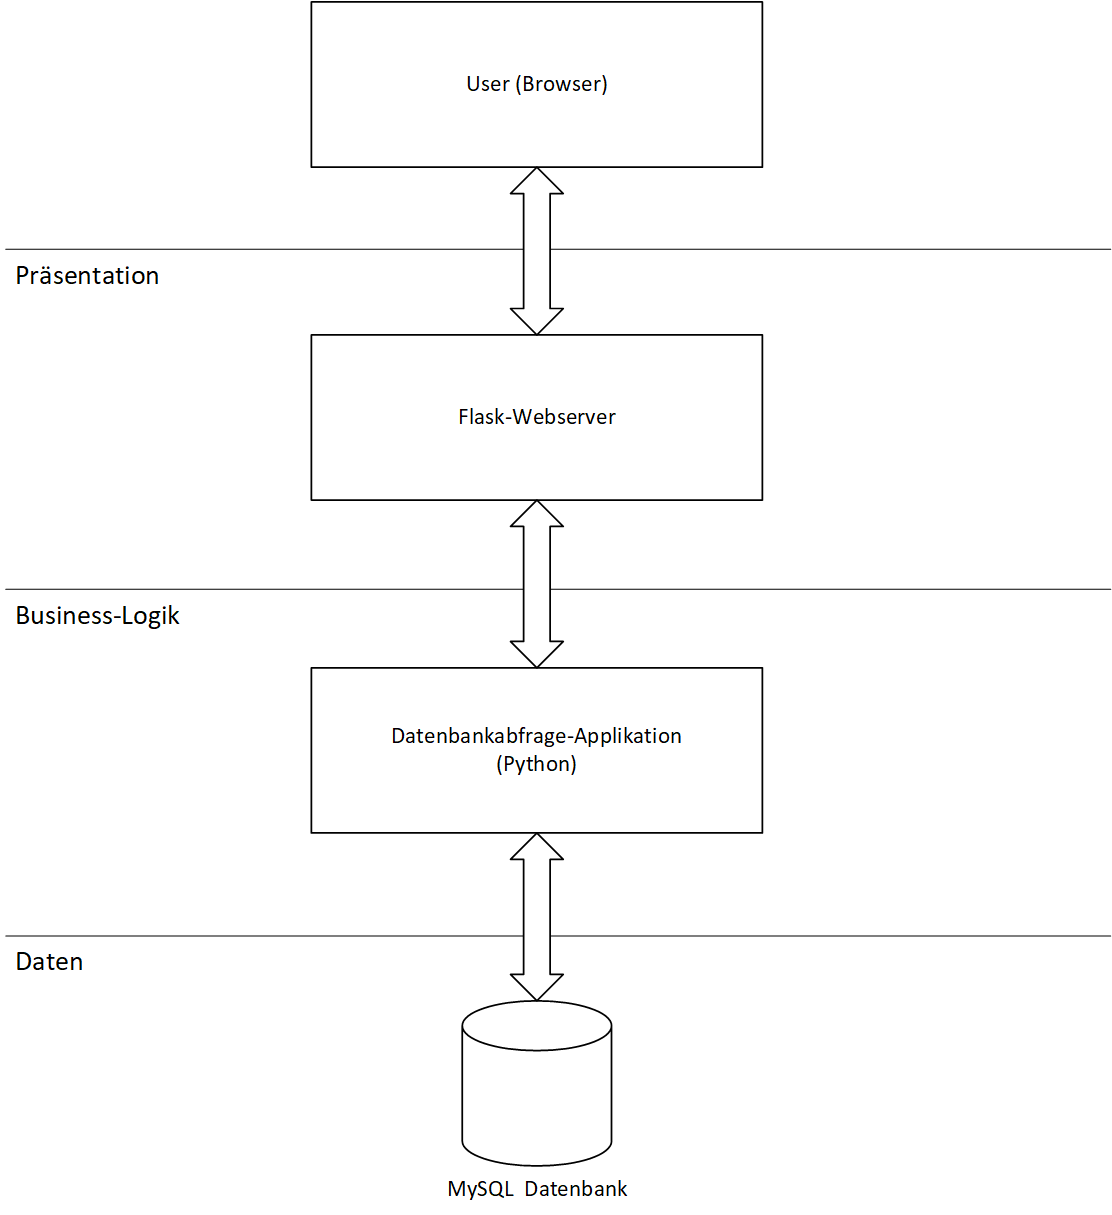
\includegraphics[width=0.9\columnwidth]{2_Datenmanagement/Bilder/ProjektArchitektur.png}
	\caption{Projektarchitektur unterteilt in Schichten.}
	\label{fig:Projektarchitektur}
\end{figure}
%\include{3_Datenmodellierung/datenmodellierung}
%\include{4_Datenbanksprache/datenbanksprache}
%\include{5_Systemarchitektur/systemarchitektur}
%\include{6_Resultate/resultate}
%\include{7_Rückblick/rückblick}
\printbibliography
%\include{9_Appendix/appendix}

%\bibliography{./bibtex/refs}
%\bibliographystyle{plain} %ieeetr}

\end{document}
